\chapter{Genes Are Not Always-On Lights}

\begin{kaichang}
Imagine accidentally cutting your finger on paper. Days later, the wound heals with exactly the right material: skin. No patch of nail, cartilage, or liver appears. Yet every nearby cell's nucleus contains the same complete DNA set, including genes for liver cells, cornea, and nails.

Other facts are equally odd. A firefly's rear glows, whereas your buttock cells do not simply have ``broken glow genes''; they do not need those blueprints at all. Cut a rose stem and plant it: cells formerly making only leaves and stems suddenly switch careers and grow roots. Exercise for three months and your arms thicken, not because muscle cells gained genes, but because the same genes changed their workload.

Different cells read entirely different passages from the same book. How do they choose pages? More importantly, \textbf{who} presses the switch? Guess first. By the end, the answer will be both simpler and subtler than ``a commander gives orders.''
\end{kaichang}

\section{One Book, Different Readings}

Begin with visible phenomena.

Your body has over two hundred cell types: neurons extend long wires, muscle cells fill with contractile fibers, and red cells discard their nuclei to make room for hemoglobin. Appearance, work, and lifespan differ enormously. Yet, with very few exceptions, every nucleus contains an identical DNA sequence, Chapter 66's three-billion-letter book.

The single-celled world shows this more directly. Gut-dwelling E. coli can consume glucose or lactose, milk sugar. Offer both and it concentrates on glucose, ignoring nearby lactose. When glucose runs out, it ``pauses'' for tens of minutes, then starts consuming lactose. A quiet internal reorganization fills that pause, an intermission before our main character enters.

Similar ``gear changes'' occur everywhere:

\begin{itemize}[itemsep=2pt]
\item Yeast entering dough ``chews glucose carefully'' through respiration while oxygen lasts, then ``gulps it'' through fermentation, releasing dough-raising carbon dioxide (Chapters 52 and 53).
\item Sunlight darkens your skin because ultraviolet increases output from melanin-making genes in melanocytes.
\item As a wound scabs, edge cells receive signals to activate proliferation genes, then brake when healing finishes.
\item Autumn leaves yellow as cells shut down chlorophyll maintenance, recovering useful nitrogen and magnesium into branches for winter.
\end{itemize}

All reflect one fact: \textbf{gene expression levels are adjustable}. Chapters 68 and 69 used ``expression'' for the whole process of transcribing DNA into RNA, translating protein, and putting it to work. Possessing a gene and using it are different things.

\section{Molecular Switches: The Lac Operon}

Zoom inside E. coli to investigate those tens of minutes of ``hesitation.''

Recall Chapter 68: transcription starts at a \textbf{promoter}, a special DNA sequence acting as a parking space for RNA polymerase. Once parked, polymerase drives along DNA, transcribing the genes it passes.

Lactose-processing machinery mainly consists of two proteins: one transports lactose into the cell, the other splits it, lactase. Conveniently, their genes sit shoulder to shoulder and share one promoter, like machines sharing a master switch. Between promoter and genes lies another special DNA stretch, the \textbf{operator}. This whole ``one switch, several genes'' apparatus is the \textbf{lac operon}; operon means an ``operating unit.''

\begin{center}
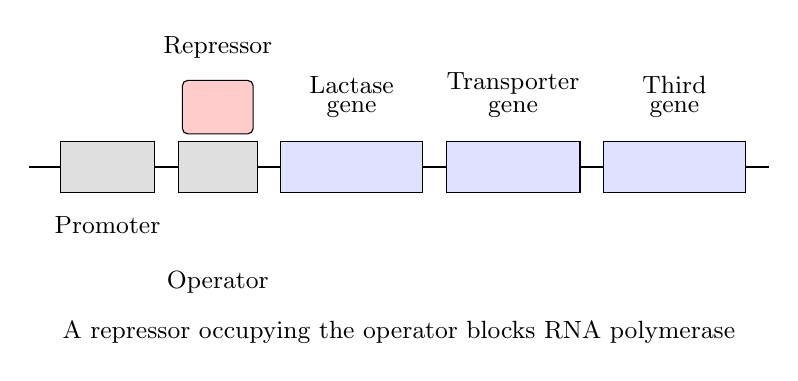
\begin{tikzpicture}[x=1cm,y=1cm]
  \draw[thick] (0,0) -- (9.4,0);
  \draw[fill=gray!25] (0.4,-0.32) rectangle (1.6,0.32);
  \node[anchor=north] at (1.0,-0.5) {\small Promoter};
  \draw[fill=gray!25] (1.9,-0.32) rectangle (2.9,0.32);
  \node[anchor=north] at (2.4,-1.2) {\small Operator};
  \draw[fill=blue!12] (3.2,-0.32) rectangle (5.0,0.32);
  \node[anchor=south] at (4.1,0.5) {\small \shortstack{Lactase\\gene}};
  \draw[fill=blue!12] (5.3,-0.32) rectangle (7.0,0.32);
  \node[anchor=south] at (6.15,0.5) {\small \shortstack{Transporter\\gene}};
  \draw[fill=blue!12] (7.3,-0.32) rectangle (9.1,0.32);
  \node[anchor=south] at (8.2,0.5) {\small \shortstack{Third\\gene}};
  \draw[fill=red!20,rounded corners=2pt] (1.95,0.42) rectangle (2.85,1.1);
  \node[anchor=south] at (2.4,1.25) {\small Repressor};
  \node at (4.7,-2.1) {\small A repressor occupying the operator blocks RNA polymerase};
\end{tikzpicture}
\end{center}

This is a human representation: box sizes and colors are not real shapes. Actual molecules are folded proteins and wound DNA.

The switch's key is a \textbf{repressor protein}, shaped to grip the operator tightly. Sitting there like a roadblock across a parking space, it prevents RNA polymerase from passing and transcribing the downstream genes. The light is off.

What happens when lactose arrives? A little incoming lactose becomes a slightly differently shaped molecule, allolactose, fitting a pocket in the repressor. Binding changes its shape so it cannot grip DNA and drops off the operator. The roadblock lifts; polymerase advances; transporter and lactase are mass-produced. The light turns on. Once lactose is exhausted, nothing occupies the pocket, the repressor returns to DNA, and the light turns off.

Notice the causal chain: nobody ``gives orders.'' Lactose and repressor bind through Chapter 22's intermolecular forces; matching shapes attract, and sufficient concentration makes binding likely. Binding changes shape, invoking Chapter 48's ``protein shape is function.'' No individual decides. The decision emerges from physical rules.

What about preferring glucose? Abundant glucose closes a second gate: a signaling molecule sensing energy status falls to low concentration, making the promoter difficult for polymerase to find. Both gates must open for maximum brightness. One asks ``is lactose present?'' and the other ``is energy scarce?''---an AND operation. Your phone chip is full of such logic gates; bacteria used them billions of years earlier.

\section{Not a Switch, but a Dimmer}

``On'' and ``off'' are useful shorthand. Real gene regulation is more like a dimmer, for two reasons.

First, \textbf{binding is probabilistic}. Repressor is not welded to DNA; it binds, falls off, and binds again. Higher lactose means its pocket spends more time occupied by inducer and less time on DNA. Transcription therefore varies in amount, not simply presence: a little more lactose gives a little more RNA per hour and more enzyme.

Second, \textbf{signal strength itself carries information}. Eukaryotic genes often have several ``parking spaces'': regulatory sequences near promoters, distant \textbf{enhancers} tens of thousands of letters away that loop back to help, and opposing \textbf{silencers}. Proteins recognizing these sites are \textbf{transcription factors}. Some help polymerase park, others block it, and others bend DNA to bring distant enhancers close. A gene listens to several factors; a factor controls hundreds of genes. This is \textbf{combinatorial regulation}. Hundreds of factors can theoretically generate astronomical numbers of ``brightness patterns,'' explaining how roughly twenty thousand genes direct over two hundred cell types.

\begin{qiaoliang}
How wide is the dimmer's range? Consider lactase. Researchers measured fewer than five molecules per E. coli cell without lactose---individual molecules, not moles. Sufficient inducer raises this to thousands, a few percent of all cellular protein. Fewer than five to thousands is roughly a thousandfold change.

A second number is striking. Each bacterium has only about ten repressor copies. Its volume is roughly one cubic micrometer, $10^{-15}$ liters. What concentration is ten molecules?
\[
\frac{10}{6.02\times 10^{23}\ \mathrm{mol^{-1}}\times 10^{-15}\ \mathrm{L}}\approx 1.7\times 10^{-8}\ \mathrm{mol/L}
\]
Seventeen billionths of a mole per liter. Precise control at that dilution depends on the repressor's extremely high affinity for the operator sequence, Chapter 48's molecular recognition at work. But ten molecules also mean those one or two seconds after detachment depend on chance. Identical bacteria consuming identical lactose may switch on minutes apart. This is the source of ``random fluctuation,'' revisited later.
\end{qiaoliang}

Regulation also loops output back onto input: \textbf{feedback}. E. coli's tryptophan-synthesis pathway is classic. Tryptophan is its final product, but when abundant, it helps a repressor hold down the pathway's own switch. More product, less production; less product, more production. Chapter 31's equilibrium shifts to oppose disturbances follow similar logic, though gene circuits execute it here. Positive feedback also exists: a product can promote its own expression, locking itself on like microphone feedback, remembering a temporary signal for a long time.

Layers of switches, dimmers, and feedback form a \textbf{gene regulatory network}. It resembles not a ladder but a subway map of interconnections. This network is the full answer to ``how genes work''; an operon is merely one especially clear station.

\section{Circuit Diagrams for Genes}

After the verbal descriptions, introduce symbols. Engineers draw electrical circuits, biologists regulatory networks, using surprisingly similar conventions: boxes or lines for genes, arrows for effects.

\begin{itemize}[itemsep=2pt]
\item An arrow $\rightarrow$ means activation. $A \rightarrow B$ means protein A brightens gene B.
\item A blunt-ended line $\dashv$ means inhibition. $A \dashv B$ means protein A dims gene B.
\end{itemize}

The lac operon's core becomes:
\[
\text{repressor} \dashv \text{lac operon}, \qquad \text{lactose} \dashv \text{repressor}
\]
Lactose inhibits the inhibitor; two negatives make a positive, so the light turns on. Tryptophan regulation becomes:
\[
\text{tryptophan} \rightarrow \text{repressor activity} \dashv \text{tryptophan-synthesis genes}
\]
An inhibitory loop: product throttles its own line, negative feedback. Developmental fate decisions that ``keep going once begun'' often appear as a self-pointing arrow, $\text{A} \rightarrow \text{A}$: positive feedback. Arrows show who influences whom and in which direction, not numerical strength. Strength depends on binding probability, the previous section's dimmer. Do not underestimate these two line types: modern systems biology feeds thousands of such arrows into computers to predict cellular behavior.

\section{Two-Stage Growth and a Nobel Prize}

\begin{zhengju}
This theory did not spring from a genius's imagination. It began with an odd curve.

In the 1940s, Jacques Monod at France's Pasteur Institute studied bacterial growth. Population versus time usually gave a smoothly rising curve. But adding both glucose and lactose yielded a strange shape: rise, plateau, rise---two steps separated by a pause. Others might have dismissed it as error; Monod insisted on asking what bacteria did during those tens of minutes.

He first excluded one explanation: bacteria were not dying and being replaced, because microscopic counts did not fall. They must instead be changing equipment. Glucose-processing enzymes were already present; lactose-processing ones had to be made. Monod called the phenomenon ``diauxic growth'' and asked how cells ``knew'' lactose had arrived.

The hard part followed. To understand a switch, change it and observe the outcome, genetics' old method since Chapter 63. Monod and François Jacob screened many switch-defective mutants: some made lactase regardless of lactose, stuck on; others never made it, stuck off. Their 1961 operon model proposed a ``repressor'' normally holding genes down until lactose released it. Stuck-on mutations represented broken repression; supplying a normal repressor gene restored the switch.

But this remained a \textbf{model}: nobody had seen the repressor inferred from switch behavior. A skeptic could suggest no repressor protein existed, only some other cause. Science had one answer: isolate it. In 1966, Gilbert and Müller-Hill did exactly that, extracting a protein that specifically gripped operator DNA and released it when a lactose derivative arrived, just as predicted. The model's ghost became a weighable molecule in a centrifuge tube, securing the theory. Monod and Jacob received the 1965 Nobel Prize for this work; protein isolation was just finished at award time, so the committee took a risk and won.

The lesson is the method: notice an unexpected step, break hypothetical switch components with mutations to test them individually, then confront the physical molecule. Until all three evidence layers aligned, the repressor remained a hypothesis awaiting confirmation.
\end{zhengju}

\begin{shiyan}
\textbf{Watch Yeast Change Gears} (suitable for home).

Materials: a small packet of dry yeast, white sugar, two identical clear mineral-water bottles, two balloons, warm water (warm but not hot to touch, around $35\,^{\circ}\mathrm{C}$; above $45\,^{\circ}\mathrm{C}$ kills yeast), a spoon, and a marker.

Steps:
\begin{enumerate}[itemsep=1pt]
\item Half-fill both bottles with warm water. Dissolve two spoonfuls of sugar in one; leave the other unsweetened as a control.
\item Add half a spoonful of dry yeast to each and swirl gently.
\item Fit balloons over the mouths and mark the starting time and state on the bottles.
\item Leave somewhere warm and observe every ten minutes for over an hour. When does inflation start, and which starts first? Does the sugared bottle reach full speed immediately or gradually accelerate?
\end{enumerate}

Observations: Yeast needs time after encountering sugar to bring fermentation to full output, so balloons often inflate slowly then faster. This resembles Monod's step: a changed menu requires new equipment. The unsweetened control helps establish that sugar drives inflation, not simply yeast meeting water.

Safety: Use only warm water; do not test a hot-water flask's temperature directly with your mouth. Afterward, pour liquid down the drain and wash bottles. Do not seal glass containers: accumulating gas can burst them.
\end{shiyan}

\textbf{Translator safety note:} Use only the specified plastic bottles with freely expandable balloons, never rigid caps or sealed glass, and do not heat or drink the cultures. An adult should supervise; keep balloons away from young children and avoid latex balloons if allergic. Follow \href{https://www.acs.org/education/celebrating-chemistry-editions/2024-ccew/science-safety-tips.html}{ACS activity precautions} and \href{https://www.cdc.gov/niosh/docs/2012-119/default.html}{NIOSH latex guidance}.

\section{Where the Model Fails}

The elegant lac operon is a \textbf{bacterial} switch. Transplant its picture directly into humans and encounter three walls.

First, eukaryotes---you, roses, flies---lack this ``one switch, several genes'' operon arrangement. Most genes have separate promoters and many transcription factors, making regulation more complex. Enhancers can sit hundreds of thousands of letters away, reaching targets through DNA folding. A bacterial roadblock-at-the-door picture does not apply here at all.

Second, DNA is not naked: it winds around histone spools and folds into chromatin (Chapter 66). Tightly wrapped DNA is inaccessible to polymerase, so eukaryotic switching largely concerns \textbf{how much DNA is exposed}. Unneeded regions are packed away, needed ones loosened. Packaging can sometimes be copied during cell division and even, in certain plants and animals where evidence remains debated, inherited across generations. Sequence stays unchanged while use changes. That is Chapter 74's epigenetics. Remember that regulation has layers, some softer than sequence but still inheritable.

Third, even in bacteria an operon is not the whole story. Every lac-circuit component connects to other circuits, with widespread consequences. ``One switch, one function'' is teaching, not daily cellular reality.

Limited models are still useful. Precisely because an operon's structure and switches are simple, engineers made it an exceptionally useful biotechnology component. Put a human insulin gene behind its promoter in E. coli; keep it off while bacteria multiply; then add inducer to the fermentation tank and switch the whole population to insulin production. Much recombinant insulin is manufactured this way (Chapter 55 covered its metabolic role; Chapter 83 explains industrial production). A basic 1961 discovery now works in pharmaceutical factories daily.

\begin{wuqu}
``Cells use needed genes; unused genes gradually degenerate and disappear.'' This confuses two levels. First, \textbf{within an individual's cells}, unused genes are switched off, their sequences intact. Rose stem cells can activate root formation after cutting, and a small plant tissue sample can regrow a whole plant in culture. Dolly is more direct: her nucleus came from an adult sheep's mammary cell, whose closed programs for making an entire sheep were reopened and executed. An off light has not been dismantled. Second, \textbf{over evolutionary time}, wholly unused traits, such as cave-fish eyes, may accumulate gene-disrupting mutations as selection relaxes maintenance. That happens over millions of years, nothing like a cell switching off, and not because a cell ``decides something is useless and discards it.'' Confusing these levels mixes regulation with mutation and development with evolution, distinctions revisited in Chapter 72 and from Chapter 76 onward.
\end{wuqu}

\section{Back to the Cut Finger}

Now answer the opening question. Wound-edge cells retain all liver and corneal genes, closed through multiple layers: missing transcription factors, silent enhancers, and packed DNA. Meanwhile, positive-feedback circuits lock in ``skin identity'': key factors promote themselves and one another, helping cells remember their identity. Healing temporarily raises repair programs---proliferation, migration, collagen secretion. Afterward, negative feedback switches proliferation off and applies brakes. Failed brakes are one source of the cancer discussed in Chapter 59.

A firefly's rear glows because luciferase genes are activated in that segment's cells. Rose cuttings root because wound-hormone signals move transcription factors into a root-making brightness pattern. Sunlight darkens skin because ultraviolet signals pass through a protein relay to melanocyte gene dimmers. The logic is shared: sequence is the book, regulation the reading. The same book supports countless readings.

A deeper flavor deserves attention: there is no commander. Switching is the statistical result of local collisions, binding, and release. Yet thousands of networked dimmers produce astonishing reliability: skin cells almost never mistakenly grow into liver. Reliability comes from redundancy, not a ruler. Multiple gates and feedback layers back each other up. This continues Volume I's theme: macroscopic certainty emerges from microscopic probability.

\section{Deeper: Flickering Lights}

\begin{tiaozhan}
Remember the roughly ten repressor molecules per bacterium? Switch states have real \textbf{randomness}. In identical bacteria sharing medium, one operator may momentarily be empty, light on, while another is occupied, light off. This is expression ``noise.''

Cells usually suppress noise, but sometimes \textbf{use} it. In Bacillus subtilis under adverse conditions, random circuit fluctuations can push a few individuals across a positive-feedback threshold into ``competence,'' a state allowing DNA uptake from outside. The population buys lottery tickets, and random winners gain alternative survival options. Embryos show an even more striking parallel: initially identical cells in certain tissues fluctuate until one crosses a threshold. Positive feedback locks in the state, and the cell inhibits neighbors from becoming the same. One randomly lit lamp helps decide who becomes a neuron and who epidermis. Fate is not entirely prewritten: some arises from dice plus self-locking. This involves feedback mathematics, including bistability and bifurcation, and can be skipped. If you wonder how randomness makes reliable patterns, it is an especially active frontier of developmental biology.
\end{tiaozhan}

A deeper question is now unavoidable. We keep saying ``gene expression'' and ``genes switched off,'' but what is a gene? A protein-making passage? Do regulatory-RNA passages count? Are enhancers and regulatory sequences part of genes? Does one DNA region spliced into several products count as one gene or several? Surprisingly, this everyday school-biology word still lacks a definition satisfying everyone. Next chapter, we operate on the word itself.

\section*{Try It Yourself}

\begin{sikaoti}
\item Use words or symbols ($\rightarrow$, $\dashv$) to map lac-operon information flow from lactose appearing in medium to rising lactase concentration, labeling each activation or inhibition. Then draw tryptophan synthesis's negative-feedback loop with the same notation.
\item Repressor detachment is probabilistic. Suppose it occupies DNA 99\% of the time without lactose and 1\% with sufficient lactose. Explain qualitatively why an intermediate concentration, such as 50\%, gives a half-bright light rather than half the cells fully on and half off. (Hint: how often can a switch change over several minutes?)
\item Propose two hypotheses for the pause in Monod's diauxic curve, including one his observation excluded. What observation would distinguish the remaining hypotheses?
\item Two cells of one rose, one petal and one root, share identical DNA but make largely different proteins. Draw material/information flow from the same DNA book through branching steps to different protein inventories. At the branch, label who reads which page.
\item Why do engineers controlling bacterial insulin production with a modified lac operon deliberately keep it normally off rather than producing at full speed continuously? Consider the energy cost from Chapter 50.
\item Cave-fish eye regression is often wrongly cited as evidence that unused genes disappear within cells. Which two timescales and levels of process are being confused?
\end{sikaoti}
